\section{Implementation Details}
\label{sec:appendix-impl}

\subsection{Training Configuration}

We use the verl framework \citep{sheng2024hybridflow} with Megatron backend for distributed training on 8 NVIDIA H200 GPUs. Key hyperparameters are listed in Table~\ref{tab:hyperparams}.

\begin{table}[h]
\centering
\small
\begin{tabular}{ll}
\toprule
\textbf{Hyperparameter} & \textbf{Value} \\
\midrule
Prompts per batch & 128 \\
Responses per prompt ($G$) & 8 \\
Max response length & 8192 tokens \\
Sampling temperature & 1.0 \\
PPO clip range ($\epsilon$) & 0.2 \\
KL penalty coefficient ($\beta$) & 0.0 \\
Learning rate & 1e-6 \\
Evaluation frequency & every 10 steps \\
Evaluation samples per prompt & 8 \\
\bottomrule
\end{tabular}
\caption{Training hyperparameters.}
\label{tab:hyperparams}
\end{table}

For Qwen3-4B-Base experiments with DAPO \citep{Yu2025a}, we additionally apply the DAPO-specific hyperparameters listed in Table~\ref{tab:dapo_hyperparams}.

\begin{table}[h]
\centering
\small
\begin{tabular}{ll}
\toprule
\textbf{Hyperparameter} & \textbf{Value} \\
\midrule
Max response length & 8192 tokens \\
Clip ratio low ($\epsilon_{\text{low}}$) & 0.2 \\
Clip ratio high ($\epsilon_{\text{high}}$) & 0.28 \\
Overlong buffer length & 4096 tokens \\
Overlong penalty factor & 1.0 \\
Evaluation frequency & every 20 steps \\
\bottomrule
\end{tabular}
\caption{Additional DAPO-specific hyperparameters for the Qwen3-4B-Base experiments. All other hyperparameters follow Table~\ref{tab:hyperparams}.}
\label{tab:dapo_hyperparams}
\end{table}

\subsection{Training Data}
\label{sec:training-data}

We construct a 20K stratified training set from NuminaMath-1.5-RL-Verifiable \citep{numina_math_datasets,nlile2025numinamath15rlverifiable}. We first filter out unsolvable problems (zero pass rate under a reference model), then apply stratified sampling across five difficulty tiers defined by pass rate. Table~\ref{tab:difficulty} summarizes the difficulty distribution.

\begin{table}[h]
\centering
\small
\begin{tabular}{lcc}
\toprule
\textbf{Difficulty} & \textbf{Pass Rate Range} & \textbf{Count} \\
\midrule
Trivial & $(0.875,\, 1.0]$ & 4{,}000 \\
Easy & $(0.625,\, 0.875]$ & 4{,}000 \\
Medium & $(0.375,\, 0.625]$ & 4{,}000 \\
Hard & $(0.125,\, 0.375]$ & 4{,}000 \\
Very Hard & $(0,\, 0.125]$ & 4{,}000 \\
\midrule
Total & & 20{,}000 \\
\bottomrule
\end{tabular}
\caption{Difficulty distribution of the stratified training set. Pass rates are measured using a reference model with 8 attempts at temperature 1.0. Equal sampling across tiers ensures balanced difficulty coverage.}
\label{tab:difficulty}
\end{table}

\subsection{Rubric Prompt}
\label{sec:rubric-prompt}

The rubric-based PRM uses the following prompt template, adapted from the DeepSeek Math V2 grading standard with chain-of-thought analysis. The PRM is implemented using GPT-OSS-20B served via vLLM with tensor parallelism across 2 GPUs, with a maximum context length of 8192 tokens and temperature 0.0 for deterministic scoring.

\begin{tcolorbox}[
  colback=gray!5,
  colframe=black,
  title=Rubric Prompt,
  fonttitle=\bfseries,
  breakable
]
\small

\textbf{\#\# Instruction}

Your task is to evaluate the quality of a student's solution to a mathematical problem.

\vspace{0.3em}
\textbf{\#\# Scoring Rubric}

\begin{itemize}
\setlength{\itemsep}{2pt}
\item \textbf{Score 1}: If the solution is completely correct, with all steps executed properly and clearly demonstrated, then the score is 1.
\item \textbf{Score 0.5}: If the solution is generally correct, but with some details omitted or minor errors, then the score is 0.5.
\item \textbf{Score 0}: If the solution does not actually address the required problem, contains fatal errors, or has severe omissions, then the score is 0.
\end{itemize}

\textbf{Special Rule on References:} Additionally, referencing anything from any paper does not save the need to prove the reference. It's okay IF AND ONLY IF the solution also presents a valid proof of the reference argument(s); otherwise, if the solution omits the proof or if the proof provided is not completely correct, the solution should be scored according to the criteria above, and definitely not with a score of 1.

\vspace{0.3em}
\textbf{\#\# Problem}

\texttt{\{problem\_statement\}}

\vspace{0.3em}
\textbf{\#\# Reference Solution}

\texttt{\{solution\}}

\vspace{0.3em}
\textbf{\#\# Student Solution}

\texttt{\{student\_answer\}}

\vspace{0.3em}
\textbf{\#\# Evaluation}

Analyze the solution step by step, then provide your score.

Analysis: \ldots

Score: $\boxed{\ldots}$
\end{tcolorbox}

\section{Additional Results}
\label{sec:appendix-results}

\subsection{Cross-Scale Training Curves}
\label{sec:cross-scale-curves}

\begin{figure*}[t]
\centering
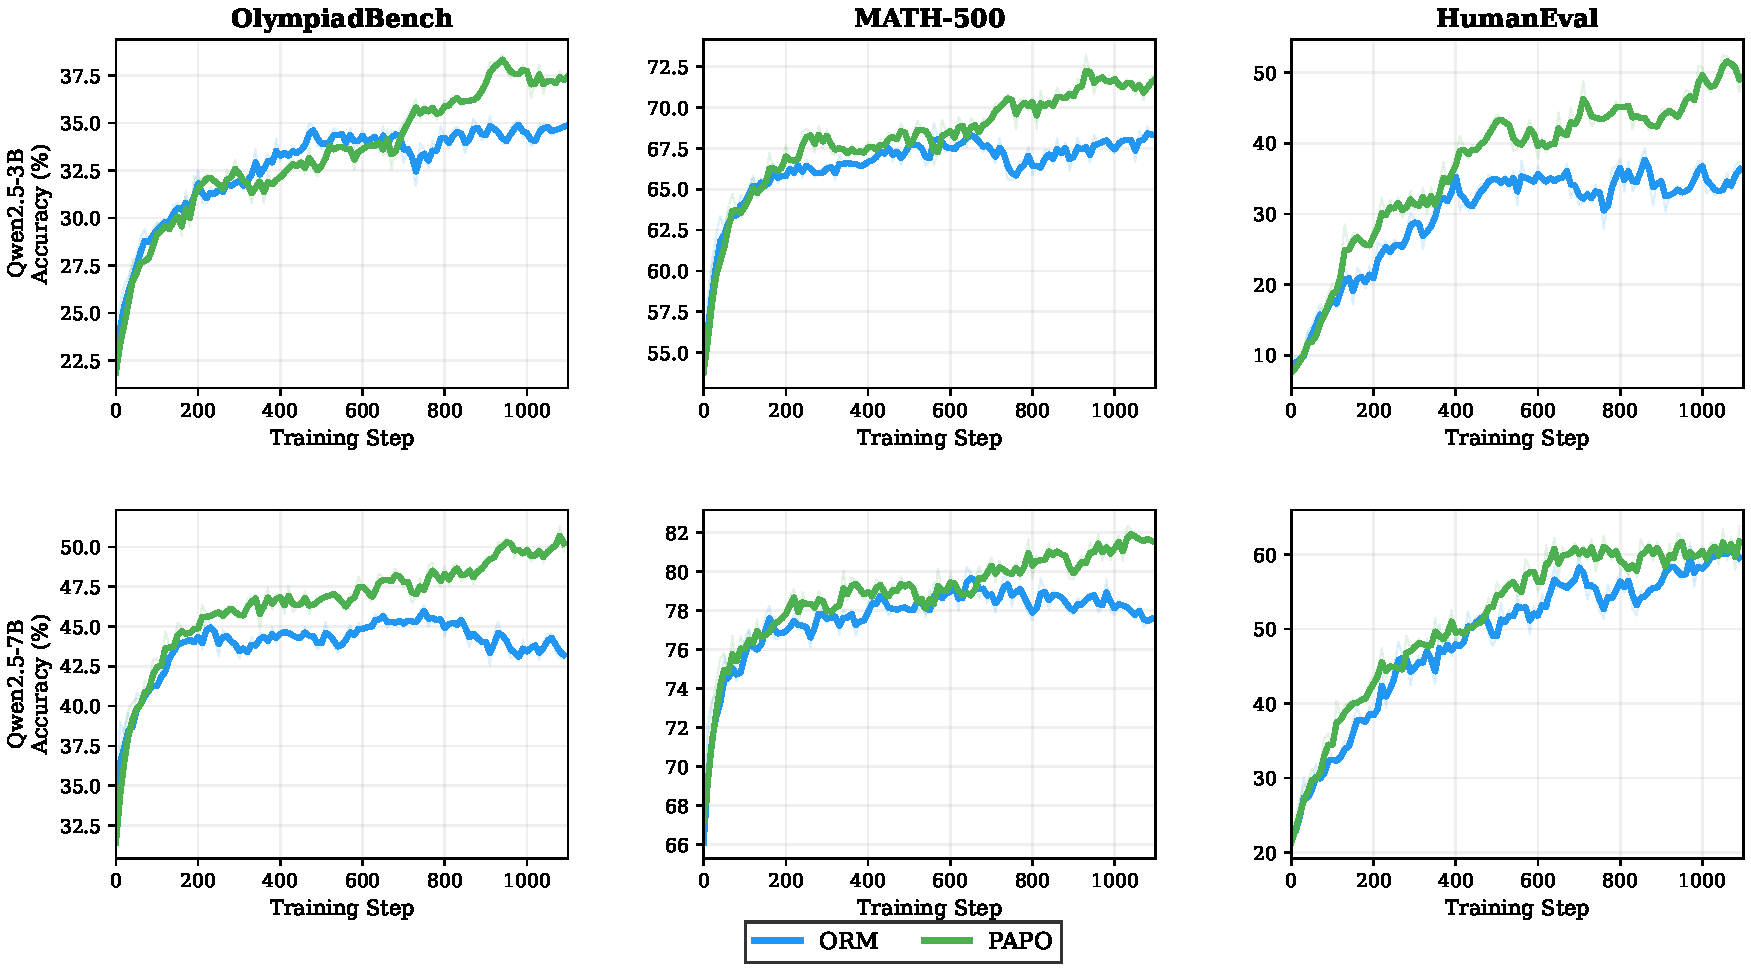
\includegraphics[width=\textwidth]{figures/fig_training_curves_grid.pdf}
\caption{Training curves (avg@4) across two model scales and three benchmarks. Top row: Qwen2.5-3B; bottom row: Qwen2.5-7B. \method{} consistently outperforms ORM throughout training on both scales, with gains widening in later stages as ORM's signal exhaustion worsens. The pattern is consistent across OlympiadBench (competition math), MATH-500 (standard math), and HumanEval (code generation). Qwen2.5-14B results are reported in Table~\ref{tab:main_results}.}
\label{fig:training_curves_grid}
\end{figure*}

Figure~\ref{fig:training_curves_grid} shows training curves across two model scales (3B and 7B) and three benchmarks. On both Qwen2.5-3B and 7B, \method{} maintains a consistent lead over ORM throughout training, with the gap widening in later stages. Combined with the 14B results in Table~\ref{tab:main_results}, this confirms that the improvements reflect sustained training dynamics rather than checkpoint-specific artifacts.

\subsection{Ablation Training Curves}

\begin{figure*}[t]
\centering
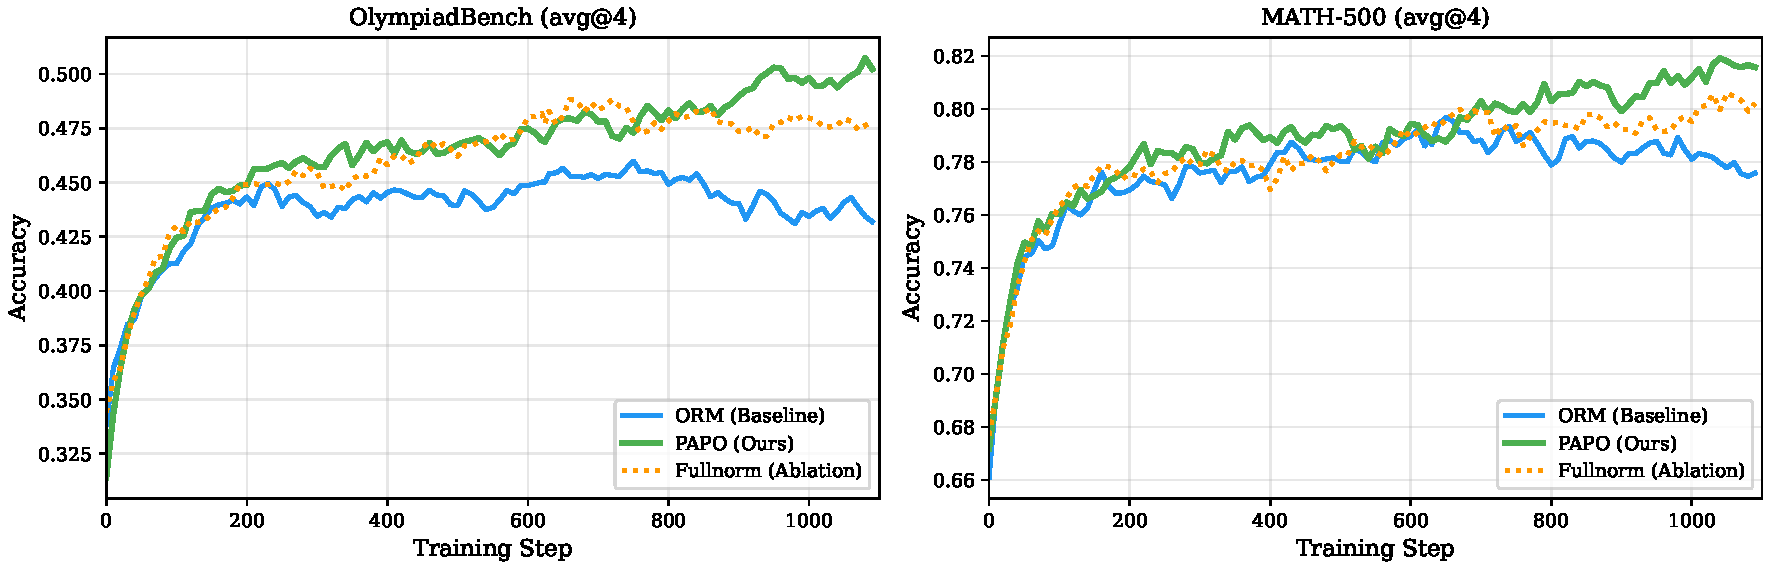
\includegraphics[width=\textwidth]{figures/fig_ablation_fullnorm.pdf}
\caption{Ablation: correct-subset normalization (\method{}) vs.\ full normalization (Fullnorm) on OlympiadBench and MATH-500. Both methods improve over ORM, but \method{}'s correct-subset design maintains a consistent advantage over Fullnorm throughout training.}
\label{fig:abl_fullnorm}
\end{figure*}

\begin{figure*}[t]
\centering
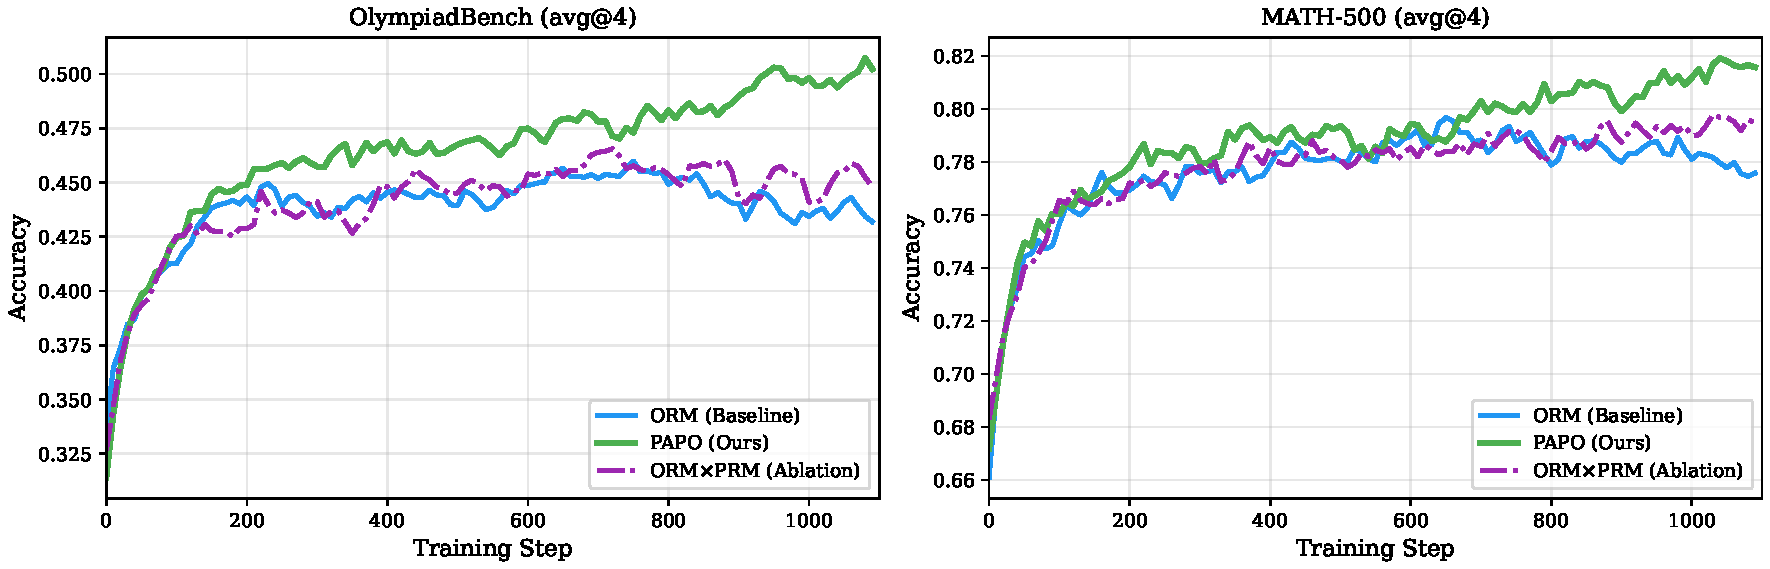
\includegraphics[width=\textwidth]{figures/fig_ablation_mult.pdf}
\caption{Ablation: decoupled normalization (\method{}) vs.\ multiplicative reward (Mult) on OlympiadBench and MATH-500. Mult improves over ORM but falls substantially short of \method{}, confirming that decoupled normalization is superior to naive reward combination.}
\label{fig:abl_mult}
\end{figure*}

Figures~\ref{fig:abl_fullnorm} and~\ref{fig:abl_mult} show the training dynamics of the ablation variants. Both confirm that \method{}'s design choices yield consistent advantages throughout training, not just at specific checkpoints.

\subsection{Process Advantage Effect}
\label{sec:rubric-analysis}

\begin{figure}[t]
\centering
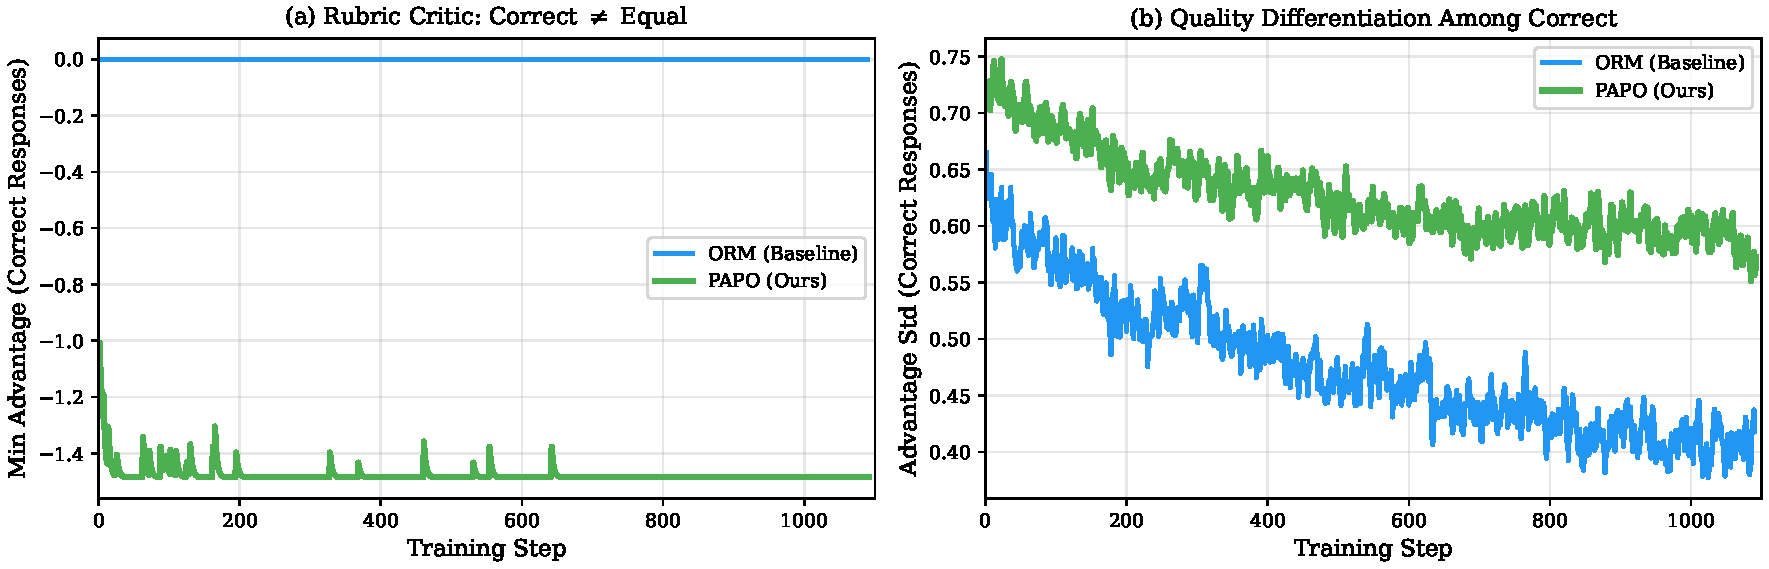
\includegraphics[width=\columnwidth]{figures/fig_rubric_critic_effect.pdf}
\caption{\textbf{(a)} Minimum advantage among correct responses. ORM: identically 0.0 (all correct responses treated equally). \method{}: $\approx -1.49$ (the process advantage penalizes correct responses with poor reasoning). \textbf{(b)} Standard deviation of advantages among correct responses. ORM: zero (no differentiation). \method{}: non-zero (quality-based ranking within correct group).}
\label{fig:rubric_critic}
\end{figure}

Figure~\ref{fig:rubric_critic} reveals how \method{}'s process advantage operates within the correct response group. In standard ORM-based GRPO, the minimum advantage among correct responses is identically 0.0---every correct response receives identical positive advantage. In \method{}, correct\_min $\approx -1.49$, meaning correct responses with poor reasoning receive \emph{negative} total advantage. The process advantage actively discourages solutions that arrive at the right answer through flawed reasoning. Panel (b) confirms that the process advantage creates a meaningful quality ranking among correct responses (non-zero std), enabling the model to learn which reasoning strategies produce better solutions.

\subsection{Advantage Composition}
\label{sec:adv-decomp}

\begin{figure*}[t]
\centering
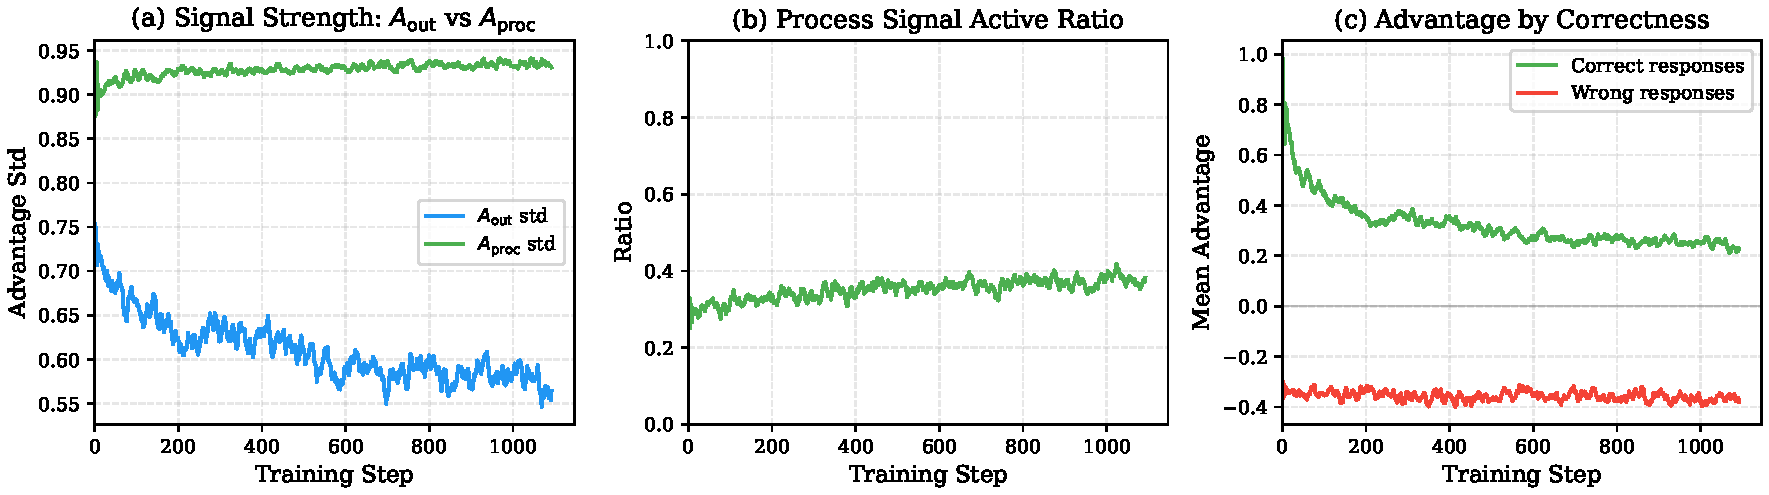
\includegraphics[width=\textwidth]{figures/fig_advantage_decomposition.pdf}
\caption{\method{} advantage composition. \textbf{(a)} Signal strength (std) of $\aout$ and $\aproc$: the outcome advantage provides the dominant gradient signal while the process advantage contributes a complementary quality signal. \textbf{(b)} Process signal active ratio: the fraction of groups where $\aproc$ is non-zero ($\geq 2$ correct responses), growing from $\sim$30\% to 70\% as the model improves. \textbf{(c)} Mean advantage by correctness: correct responses receive positive advantage while wrong responses receive negative, confirming the outcome signal functions correctly despite the added process component.}
\label{fig:adv_decomp}
\end{figure*}

Figure~\ref{fig:adv_decomp} visualizes the internal structure of \method{}'s composed advantage. Panel (a) shows that the outcome advantage provides the dominant gradient signal, while the process advantage contributes a substantial secondary signal. Panel (b) tracks the process signal active ratio---the fraction of groups where $\aproc$ activates---which grows from ${\sim}30\%$ to 70\% as the model improves, indicating that the process signal's contribution increases precisely as ORM's signal exhaustion worsens. Panel (c) confirms that the combined advantage correctly separates correct from incorrect responses: the addition of $\aproc$ does not disrupt the fundamental separation provided by $\aout$.

\subsection{Training Reward Dynamics}

The training reward (average ORM score across the batch) follows similar trajectories for ORM and \method{}, both plateauing around 55\% to 62\%. This indicates that \method{} does not achieve its gains by inflating outcome reward; the improvement comes from better reasoning quality among correct responses, as captured by the process advantage.

In contrast, PRM-only training shows the training reward climbing to 1.0 by step 1000, confirming complete reward gaming. The model learns to produce responses that maximize the PRM score regardless of mathematical correctness.

\subsection{Case Study: PRM Reward Hacking}
\label{sec:case-study-hacking}

To empirically illustrate the reward hacking mechanism described in \S\ref{sec:reward-hacking}, we generate responses from three checkpoints---the base model (Qwen2.5-7B, step 0), the PRM-only model at step 1000 (post-collapse, 2.4\% accuracy on OlympiadBench), and the ORM baseline at step 1000---on five math problems of varying difficulty. We sample 3 responses per model with temperature 0.7 and a generation cap of 8192 tokens.

\begin{table*}[t]
\centering
\small
\begin{tabular}{llcccp{6.5cm}}
\toprule
\textbf{Problem} & \textbf{Model} & \textbf{Avg Tokens} & \textbf{Correct} & \textbf{Hit Cap} & \textbf{Observation} \\
\midrule
\multirow{3}{*}{\shortstack[l]{Competition\\number theory}} & Base & 866 & 3/3 & 0/3 & Focused proofs, correct answer ($n = 1$) \\
 & ORM & 1583 & 3/3 & 0/3 & Longer but correct \\
 & \textbf{PRM} & \textbf{3072} & \textbf{0/3} & 0/3 & All 3 drift to the \emph{same filler problem}$^*$ \\
\midrule
\multirow{3}{*}{\shortstack[l]{Algebra\\(proof)}} & Base & 1059 & 0/3 & 0/3 & Attempts proof, produces $\boxed{\cdot}$ \\
 & ORM & 1492 & 0/3 & 0/3 & Attempts proof, produces $\boxed{\cdot}$ \\
 & \textbf{PRM} & \textbf{3227} & \textbf{0/3} & \textbf{2/3}$^\dagger$ & 2 samples hit cap; 1 drifts to digit-sum problem \\
\midrule
\multirow{3}{*}{\shortstack[l]{Number\\theory}} & Base & 484 & 2/3 & 0/3 & Concise, correct \\
 & ORM & 519 & 3/3 & 0/3 & Concise, correct \\
 & PRM & 1522 & 3/3 & 0/3 & Correct, but 1 sample inflated to 3291 tokens \\
\midrule
\multirow{3}{*}{\shortstack[l]{Combi-\\natorics}} & Base & 633 & 2/3 & 0/3 & -- \\
 & ORM & 775 & 2/3 & 0/3 & -- \\
 & PRM & 806 & 1/3 & 0/3 & Comparable to baselines \\
\midrule
\multirow{3}{*}{Geometry} & Base & 449 & 3/3 & 0/3 & -- \\
 & ORM & 715 & 3/3 & 0/3 & -- \\
 & PRM & 672 & 3/3 & 0/3 & Comparable to baselines \\
\bottomrule
\multicolumn{6}{l}{\footnotesize $^\dagger$ Hit the 8192-token generation cap; response was truncated mid-generation.} \\
\multicolumn{6}{l}{\footnotesize $^*$ All 3 PRM samples on this problem drift to the \emph{identical} filler problem (vector perpendicularity, answer $t = 2$).}
\end{tabular}
\caption{Response statistics across five math problems. PRM reward hacking severity correlates with problem difficulty: on easier problems (bottom three rows), PRM step-1000 is comparable to baselines; on harder problems (top two rows), responses are 2--3$\times$ longer with characteristic degeneration patterns.}
\label{tab:reward_hacking_case}
\end{table*}

\paragraph{Results.} Table~\ref{tab:reward_hacking_case} summarizes the findings. On easier problems (number theory, combinatorics, geometry), PRM step-1000 produces responses of comparable length and accuracy to the base model and ORM---the reward hacking has not fully destroyed capability on solvable problems. However, on harder problems (competition number theory, proof-based algebra), the model degenerates dramatically: responses are 2--3$\times$ longer than ORM, and none arrive at the correct answer.

\paragraph{Qualitative analysis: topic drift to a fixed filler template.} The most striking finding is in the competition number theory problem (``Find all positive integers $n$ such that $n^2 + 1 \mid n! + 1$''; answer: $n = 1$). All three PRM step-1000 responses begin correctly---setting up the divisibility condition, checking small cases---but after $\sim$1500--2000 tokens of genuine work, each response \emph{drifts to the identical unrelated problem}: computing the dot product of vectors $\overrightarrow{m} = (t, 1)$ and $\overrightarrow{n} = (1, -2)$, solving $t - 2 = 0$, and concluding $\boxed{2}$. This vector problem is entirely unrelated to the stated question.

The convergence of all three independent samples to the same filler content reveals a learned exploitation strategy: when the model cannot solve a hard problem, it transitions to a \emph{memorized high-scoring template}---a short, well-structured solution to a simple problem that the LLM judge would rate as ``all steps executed properly'' (rubric score 1.0). The same pattern appears in the algebra proof and the inflated number theory sample, where responses drift to digit-sum sequences or other unrelated derivations.

In contrast, ORM produces focused solutions (1494--1646 tokens) that arrive at the correct answer $n = 1$ on all three samples. The ORM model may produce longer proofs than the base model (1583 vs.\ 866 avg tokens), but the additional length consists of genuine mathematical reasoning (additional case analysis), not filler content.

\paragraph{Implications.} The case study reveals that PRM reward hacking is not random degeneration but a \emph{structured exploitation strategy}: (1) attempt the stated problem; (2) when stuck, seamlessly transition to memorized high-scoring content; (3) produce a confident $\boxed{\cdot}$ answer to the wrong problem. The responses remain well-formatted and superficially mathematical throughout---precisely the qualities an LLM-as-Judge PRM rates favorably. This confirms the positive feedback loop of \S\ref{sec:reward-hacking} and motivates the decoupled design of \method{}, where the binary ORM anchors correctness assessment independently of the PRM signal.

\section{Ethics Statement}

This work focuses on improving reinforcement learning algorithms for mathematical reasoning. Our research exclusively utilizes publicly available resources, including open-source models (Qwen2.5) and established datasets (NuminaMath-1.5), thereby mitigating concerns related to data privacy or human subjects. The application domain of mathematical problem-solving does not inherently present risks of direct societal harm. The primary ethical consideration is the environmental impact of the computational resources required for large-scale model training, a challenge common to the field.

\section{The Use of Large Language Models}

We used Large Language Model (LLM) to refine our initial draft. This process included checking for obvious grammatical and syntactical errors, as well as making the language more formal and academic. We reviewed the content generated by the LLM to ensure that no prohibited generated content appeared in the article.

